\documentclass{article}

\usepackage{times}
\usepackage{amsmath}
\usepackage{amsthm}
\usepackage{amssymb}
\usepackage{latexsym}
\usepackage{fullpage}
\usepackage[shortlabels]{enumitem}
\usepackage[utf8]{inputenc}
\usepackage{hyperref}
\usepackage{fancyvrb}
\usepackage{minted}
\usepackage{graphicx}
\usepackage{fancyhdr}
\usepackage[affil-it]{authblk}
\usepackage[headsep=14pt,headheight=14pt]{geometry}

\hypersetup{
    pdftitle={Problem Set I}
}

\setlength{\parskip}{.1in}
\setlength{\headheight}{15pt}
\setlength{\topmargin}{0pt}

\pagestyle{fancy}
\lhead{MATH 470: Communications and Cryptography}
\rhead{Texas A\&M University}
\cfoot{\thepage}

\title{\vspace{-2.5cm}Homework I}
\author{\vspace{-0.2cm} Huy Quang Lai\\132000359}
\affil{Texas A\&M University}
\date{\vspace{-0.5cm}30 August 2022}

\begin{document}
\maketitle
\begin{center}
\rule{\textwidth}{.1pt}
{\large
An Aggie does not lie, cheat or steal.\\
Nor does an Aggie tolerate those who do.
}
\end{center}

\section*{Problem 1}
Encrypted Text:\\
EREKK MIHSI WRSXP MIGLI EXSVW XIEPS VXSPI VEXIX LSWIA LSHS

\noindent
Decrypted Text:\\
A shift of the encoded message by $4\leftarrow$ or by $22\rightarrow$ would decode the message\\
ANAGG IEDOE SNOTL IECHE ATORS TEALO RTOLE RATET HOSEW HODO

\noindent
This message can be further parsed into the following:\\
An Aggie does not lie cheat or steal or tolerate those who do

\section*{Problem 2}
Raw Text: ``The gold is hidden in the garden"\\
Encrypted Text: ``IBXFE PAQLB QAAXW QWIBX FSVAX W"

\section*{Problem 3}
\begin{proof}
Prove that if $a|b$ and $b|a$, then $a=\pm b$\\
By definition $\exists x,y\in\mathbb{Z}$ such that $a=bx$ and $b=ay$\\
$a = bx \Rightarrow a = ayx$\\
Dividing both sides by $a$ results in:\\
$1 = yx$

\noindent
Since both $x$ and $y$ are integers and their product is 1, $x=y=\pm 1$\\
Using this result in the equation for $a$ gives:\\
$a=\pm b$
\end{proof}

\newpage
\section*{Problem 4}
$\gcd(291,252)$
\begin{flalign*}
292 &= 1*252+40 &\\
252 &= 6*40+12 &\\
40 &= 3*12+4 &\\
12 &= 3*4+0 &
\end{flalign*}
$\gcd(291,252)=3$

\section*{Problem 5}
\subsection*{Part a}
\begin{proof}
Suppose that there are integers $u$ and $v$ satisfying $au+bv=1$. Prove that $gcd(a,b)=1$\\
Let $g=\gcd(a,b)$. Then $\exists x,y\in\mathbb{Z}$ such that $a=gx\land b=gy$\\
Substituting this into the given equation $au+bv=1$ results in:
\[
1=au+bv=gxu+gyv=g(xu+yv)
\]

\noindent
$u,v,x,y\in\mathbb{Z}\rightarrow(xu+yv)\in\mathbb{Z}$\\
As a result of the previous statement:\\
$g|1$\\
This requires that $g=1$.
\end{proof}

\newpage
\subsection*{Part b}
Suppose that there are integers $u$ and $v$ satisfying $au+bv=6$. Is it necessarily true that $\gcd(a,b)=6$? If not, give a specific counterexample, and describe in general all of the possible values of $\gcd(a,b)$?

\noindent
$au+bv=6$ does not imply that $\gcd(a,b)=6$.\\
Counterexample: $a=3,b=2$
\[a\cdot(6)+b\cdot(-6)=6\]
but $\gcd(a,b)=1$

\noindent
In general, if $au+by=c$ has a solution, then $\gcd(a,b)|c$.\\
Let $g=\gcd(a,b)$. Divide $c$ by $g$ with remainder $r$ such that
\[c=gq+r \textrm{ with } 0\leq r< g\]
We know that we can find a solution to $g=ax+by$, so we get
\[au+bv=c=gq+r=(ax+by)q+r\]
Rearranging this statement results in:
\[a(u-xq)+b(v-yq)=r\]

\noindent
The left hand side is divisible by $g$ since $\gcd(a,b)=g$. Therefore, $g|r$. But the only $r$ that can satisfy both $0\leq r < g$ and $g|r$ is $r=0$. This results in $c=gq$. This implies that $\gcd(a,b)|c$

\newpage
\section*{Problem 6}
\begin{minted}{python}
def gcd(a: int, b: int):
    if a == 0:
        return b
    if b == 0:
        return a
    return gcd(b, a % b)


def main():
    a = 1234567890123456789012345678901234567890123456789012345678901234567890123456789
    b = 234567890123456789012345678901234567890123456789012345678901234567890123456789

    print("gcd(a,b) =", gcd(a, b))


if __name__ == "__main__":
    main()
\end{minted}

\begin{figure}[ht!]
    \centering
    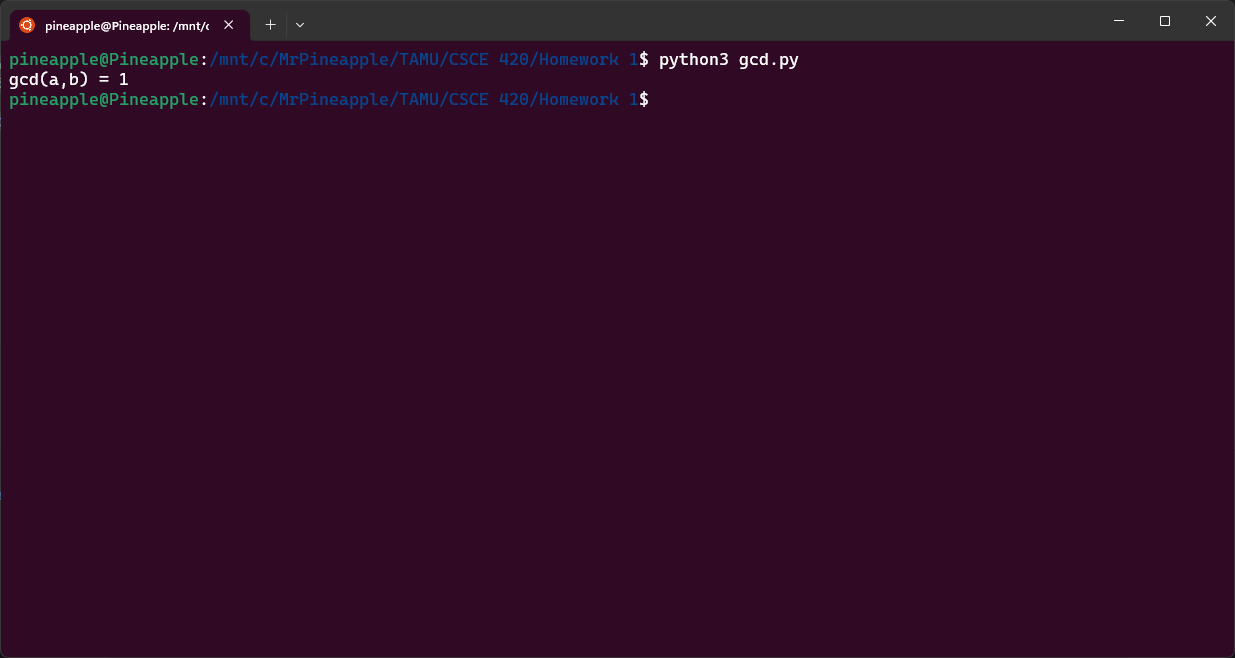
\includegraphics[width=\textwidth]{Problem 6.png}
    \caption{Output of the Code}
\end{figure}

\end{document}
